% Figure 2 of docs/expert_companion.md: the dummy input and the planted input,
% which differ at exactly two places. Build with tools/render_papers.py.
\documentclass[tikz,border=4pt]{standalone}
\usepackage{amsmath,amssymb}
\usetikzlibrary{arrows.meta,calc}
\definecolor{one}{RGB}{226,232,240}
\definecolor{zero}{RGB}{40,40,40}
\definecolor{win}{RGB}{176,58,46}
\definecolor{addr}{RGB}{40,90,150}
\begin{document}
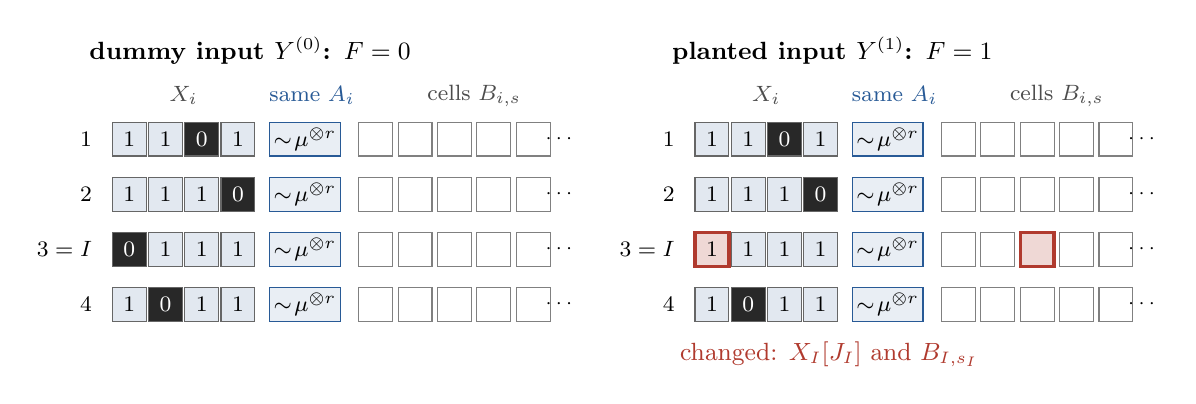
\begin{tikzpicture}[
  font=\small,
  bit/.style={draw=black!60, minimum width=4.3mm, minimum height=4.3mm,
              inner sep=0pt, font=\footnotesize},
  cell/.style={draw=black!50, fill=white, minimum width=4.3mm,
               minimum height=4.3mm, inner sep=0pt},
  >={Stealth[length=2mm]}]
% #1 x-offset, #2 panel name prefix, #3 planted? (0/1)
\newcommand{\panel}[3]{%
  \foreach \row/\z/\lab in {1/3/{1},2/4/{2},3/1/{3=I},4/2/{4}} {
    \pgfmathsetmacro{\y}{-0.7*\row}
    \node[anchor=east, font=\footnotesize] at (#1-0.12,\y) {$\lab$};
    \foreach \c in {1,...,4} {
      \ifnum\c=\z
        \ifnum#3=1 \ifnum\row=3
          \node[bit, fill=win!20, draw=win, very thick] (#2\row-\c)
            at (#1+0.46*\c-0.23,\y) {1};
        \else
          \node[bit, fill=zero, text=white] (#2\row-\c) at (#1+0.46*\c-0.23,\y) {0};
        \fi \else
          \node[bit, fill=zero, text=white] (#2\row-\c) at (#1+0.46*\c-0.23,\y) {0};
        \fi
      \else
        \node[bit, fill=one] (#2\row-\c) at (#1+0.46*\c-0.23,\y) {1};
      \fi}
    \node[draw=addr, fill=addr!10, minimum width=9mm, minimum height=4.3mm,
          inner sep=0pt, font=\footnotesize] at (#1+2.46,\y) {$\sim\!\mu^{\otimes r}$};
    \foreach \c in {1,...,5} {
      \ifnum#3=1 \ifnum\row=3 \ifnum\c=3
        \node[cell, fill=win!20, draw=win, very thick] (#2cell) at (#1+2.86+0.5*\c,\y) {};
      \else \node[cell] at (#1+2.86+0.5*\c,\y) {}; \fi
      \else \node[cell] at (#1+2.86+0.5*\c,\y) {}; \fi
      \else \node[cell] at (#1+2.86+0.5*\c,\y) {}; \fi}
    \node[font=\scriptsize] at (#1+5.71,\y) {$\cdots$};
  }
  \node[font=\footnotesize, black!70] at (#1+0.92,-0.15) {$X_i$};
  \node[font=\footnotesize, addr] at (#1+2.55,-0.15) {same $A_i$};
  \node[font=\footnotesize, black!70] at (#1+4.61,-0.15) {cells $B_{i,s}$};
}
\panel{0}{d}{0}
\panel{7.4}{p}{1}
\node[font=\small\bfseries, anchor=west] at (-0.4,0.42) {dummy input $Y^{(0)}$: $F=0$};
\node[font=\small\bfseries, anchor=west] at (7.0,0.42) {planted input $Y^{(1)}$: $F=1$};
% legend for the two changed locations
\node[win, font=\small, anchor=north west, align=left] at (7.1,-3.15)
  {changed: $X_I[J_I]$ and $B_{I,s_I}$};
\end{tikzpicture}
\end{document}
